\documentclass[aspectratio=169]{beamer}

% ---------- ENCODING & FONTS ----------
\usepackage[utf8]{inputenc}
\usepackage[T1]{fontenc}

% ---------- THEME & LOOK ----------
\usetheme{Madrid}
\usecolortheme{seahorse}
\usefonttheme{professionalfonts}
\setbeamertemplate{navigation symbols}{}
\setbeamercovered{transparent}
\setbeamertemplate{itemize items}[circle]
\setbeamertemplate{enumerate items}[default]
\setlength{\parskip}{0.25em}

% ---------- COLORS ----------
\definecolor{accent}{RGB}{0,92,184}
\definecolor{soft}{RGB}{233,244,255}
\definecolor{canadared}{RGB}{196,30,58}
\definecolor{leafgreen}{RGB}{0,130,80}
\definecolor{goldenrod}{RGB}{218,165,32}
\definecolor{deeporange}{RGB}{220,90,20}
\definecolor{demandblue}{RGB}{30,100,200}
\definecolor{supplyred}{RGB}{190,40,40}
\definecolor{eqgreen}{RGB}{20,140,60}
\definecolor{shiftpurple}{RGB}{130,50,180}
\definecolor{lightred}{RGB}{245,210,210}
\setbeamercolor{structure}{fg=accent}
\setbeamercolor{title}{fg=white,bg=accent}
\setbeamercolor{frametitle}{fg=accent}
\setbeamercolor{block title}{bg=accent!12,fg=accent}
\setbeamercolor{block body}{bg=soft}

% ---------- PACKAGES ----------
\usepackage{booktabs}
\usepackage{amsmath, amssymb}
\usepackage{array}
\usepackage{multirow}
\usepackage{hyperref}
\usepackage{tikz}
\usepackage{pgfplots}
\pgfplotsset{compat=1.18}
\usetikzlibrary{arrows.meta, positioning, calc}
\hypersetup{colorlinks=true,linkcolor=accent,urlcolor=accent}

% ---------- SAFE TRANSITION FALLBACK ----------
\makeatletter
\@ifundefined{transfade}{\newcommand{\transfade}[1][]{}}{}
\makeatother

% ---------- TITLE ----------
\title{\textbf{Where Prices Come From:\\The Interaction of Supply and Demand}}
\subtitle{{\large ECON 101 -- Principles of Macroeconomics}}
\author{Muhebullah Karimzada}
\date{Spring 2026}

% ============================================================
\begin{document}
% ============================================================

\begin{frame}[plain]
  \titlepage
\end{frame}

\begin{frame}{Chapter Outline}
\transfade
\begin{itemize}[<+->]
  \item \textbf{3.1} The Demand Side of the Market
  \item \textbf{3.2} The Supply Side of the Market
  \item \textbf{3.3} Market Equilibrium: Putting Buyers and Sellers Together
  \item \textbf{3.4} The Effect of Demand and Supply Shifts on Equilibrium
\end{itemize}
\end{frame}

% ============================================================
\section{3.1 The Demand Side of the Market}
% ============================================================

\begin{frame}{3.1 Learning Objective}
\transfade
\begin{block}{Goal}
Discuss the variables that influence demand.
\end{block}
\begin{itemize}[<+->]
  \item We begin by investigating how \textbf{buyers} behave.
  \item \textbf{Market demand:} the demand by all consumers of a given good or service.
  \item Key tools: demand schedule and demand curve.
  \item Running example: the market for \textbf{Tim Hortons medium coffee} in Canada.
\end{itemize}
\end{frame}

%--- FIG 3.1: Demand schedule + demand curve ---
\begin{frame}{Figure 3.1 -- Demand Schedule and Demand Curve}
\begin{columns}
\column{0.38\textwidth}
\centering
{\small\bfseries Tim Hortons Medium Coffee\\Demand Schedule}
\vspace{0.5em}

\renewcommand{\arraystretch}{1.4}
\begin{tabular}{cc}
\toprule
\textbf{\color{demandblue}Price} & \textbf{\color{demandblue}Qty Demanded}\\
(\$/cup) & (M cups/week)\\
\midrule
\$3.00 & 10 \\
\$3.50 & 9 \\
\$4.00 & 8 \\
\$4.50 & 7 \\
\$5.00 & 6 \\
\bottomrule
\end{tabular}
\vspace{0.5em}

{\scriptsize Source: Illustrative; based on\\Statistics Canada CPI data}

\column{0.62\textwidth}
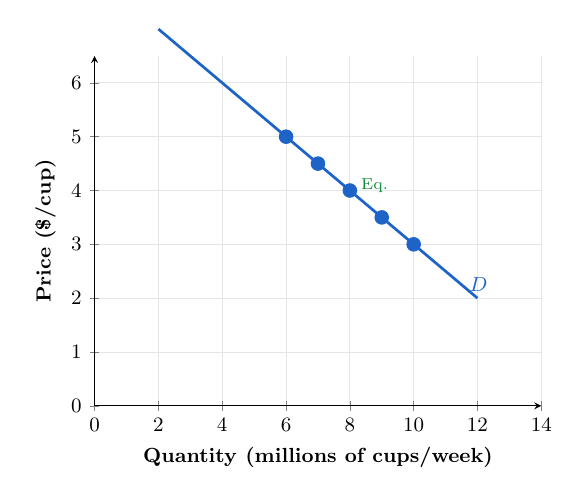
\begin{tikzpicture}[scale=0.82]
  \begin{axis}[
    width=8.5cm, height=7cm,
    xlabel={\textbf{Quantity} (millions of cups/week)},
    ylabel={\textbf{Price} (\$/cup)},
    xmin=0, xmax=14,
    ymin=0, ymax=6.5,
    xtick={0,2,4,6,8,10,12,14},
    ytick={0,1,2,3,4,5,6},
    tick label style={font=\small},
    label style={font=\small\bfseries},
    axis lines=left,
    grid=major, grid style={gray!20},
    clip=false,
  ]
  % Demand line: P = -0.5Q + 8  (Q from 0 to 16)
  \addplot[very thick, color=demandblue, domain=2:12, samples=2]
    {-0.5*x + 8};
  \node[font=\small\bfseries, color=demandblue, right] at (axis cs:11.5,2.25) {$D$};
  % Data points
  \addplot[mark=*, mark size=3pt, color=demandblue]
    coordinates {(10,3)(9,3.5)(8,4)(7,4.5)(6,5)};
  % Equilibrium label
  \node[font=\scriptsize, color=eqgreen, right] at (axis cs:8.1,4.1) {Eq.};
  \end{axis}
\end{tikzpicture}
\end{columns}
\end{frame}

\begin{frame}{Demand Schedule and Demand Curve: Key Concepts}
\transfade
\begin{itemize}[<+->]
  \item \textbf{Demand schedule:} a table showing the relationship between the \textbf{price} and the \textbf{quantity demanded}.
  \item \textbf{Demand curve:} a curve showing the same relationship graphically.
  \item When drawing the demand curve, we hold all other factors constant --- \textbf{ceteris paribus}.
  \item \textbf{Ceteris paribus:} ``all else equal'' --- when analyzing price and quantity demanded, other variables are held constant.
\end{itemize}
\end{frame}

\begin{frame}{The Law of Demand}
\transfade
\begin{itemize}[<+->]
  \item \textbf{Quantity demanded:} the amount of a good a consumer is willing and able to purchase at a given price.
  \item \textbf{Law of demand:}
  \begin{itemize}[<+->]
    \item Holding everything else constant, when the price of a product \alert{falls}, the quantity demanded \alert{increases}.
    \item When the price \alert{rises}, the quantity demanded \alert{decreases}.
  \end{itemize}
  \item \textbf{Canadian data:} When Tim Hortons raised medium coffee prices by $\approx$10\% in 2022--2023, same-store transaction counts fell in the short run (Restaurant Brands International earnings, 2023).
\end{itemize}
\end{frame}

\begin{frame}{What Explains the Law of Demand?}
\transfade
\begin{itemize}[<+->]
  \item When the price of a good falls, two key effects occur:
  \begin{itemize}[<+->]
    \item \textbf{Substitution effect:} consumers substitute toward the good whose price has fallen.
    \item \textbf{Income effect:} consumers have more real purchasing power, which raises quantity demanded.
  \end{itemize}
  \item \textbf{Substitution effect:} the change in quantity demanded resulting from a change in price relative to other goods, \emph{holding purchasing power constant}.
  \item \textbf{Income effect:} the change in quantity demanded resulting from a price change affecting consumers' \emph{purchasing power}.
\end{itemize}
\end{frame}

\begin{frame}{Canadian Example: Substitution and Income Effects}
\transfade
\small
\begin{itemize}[<+->]
  \item Suppose Tim Hortons medium coffee falls from \$4.00 to \$3.00.
  \item \textbf{Substitution effect:}
  \begin{itemize}[<+->]
    \item Coffee is now cheaper relative to Starbucks lattes, Red Bull, or tea --- consumers substitute toward Tim Hortons coffee.
  \end{itemize}
  \item \textbf{Income effect:}
  \begin{itemize}[<+->]
    \item A daily coffee drinker saves $\approx$\$365/year --- that extra real income allows more cups per week.
  \end{itemize}
\end{itemize}
\end{frame}

%--- FIG 3.2: Shifting the demand curve ---
\begin{frame}{Figure 3.2 -- Shifting the Demand Curve}
\begin{center}
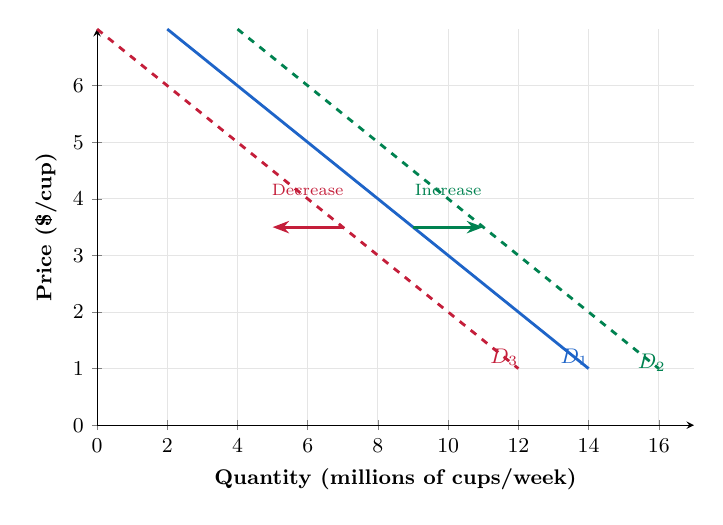
\begin{tikzpicture}[scale=0.85]
  \begin{axis}[
    width=10.5cm, height=7.5cm,
    xlabel={\textbf{Quantity} (millions of cups/week)},
    ylabel={\textbf{Price} (\$/cup)},
    xmin=0, xmax=17,
    ymin=0, ymax=7,
    xtick={0,2,4,6,8,10,12,14,16},
    ytick={0,1,2,3,4,5,6},
    tick label style={font=\small},
    label style={font=\small\bfseries},
    axis lines=left,
    grid=major, grid style={gray!20},
    clip=false,
  ]
  % D1 original: P = -0.5Q + 8
  \addplot[very thick, color=demandblue, domain=2:14, samples=2]
    {-0.5*x + 8};
  \node[font=\small\bfseries, color=demandblue] at (axis cs:13.6,1.2) {$D_1$};
  % D2 increase: P = -0.5Q + 9 (shifts right by 2)
  \addplot[very thick, color=leafgreen, domain=4:16, samples=2, dashed]
    {-0.5*x + 9};
  \node[font=\small\bfseries, color=leafgreen] at (axis cs:15.8,1.1) {$D_2$};
  % D3 decrease: P = -0.5Q + 7 (shifts left by 2)
  \addplot[very thick, color=canadared, domain=0:12, samples=2, dashed]
    {-0.5*x + 7};
  \node[font=\small\bfseries, color=canadared] at (axis cs:11.6,1.2) {$D_3$};
  % Arrows
  \draw[-{Stealth[length=7pt]}, very thick, color=leafgreen]
    (axis cs:9,3.5) -- (axis cs:11,3.5);
  \node[font=\scriptsize, color=leafgreen] at (axis cs:10,4.15) {Increase};
  \draw[-{Stealth[length=7pt]}, very thick, color=canadared]
    (axis cs:7,3.5) -- (axis cs:5,3.5);
  \node[font=\scriptsize, color=canadared] at (axis cs:6,4.15) {Decrease};
  \end{axis}
\end{tikzpicture}
\end{center}
\end{frame}

\begin{frame}{Shifts in Demand: Key Distinction}
\transfade
\begin{itemize}[<+->]
  \item A change in something \textbf{other than price} causes the \textbf{entire demand curve to shift}.
  \item $D_1 \to D_2$ (right): an \alert{increase in demand} --- more coffee demanded at every price.
  \item $D_1 \to D_3$ (left): a \alert{decrease in demand} --- less coffee demanded at every price.
  \item The quantity demanded changes at \textbf{every possible price} when the curve shifts.
\end{itemize}
\end{frame}

\begin{frame}{Variables That Shift Market Demand}
\transfade
\begin{itemize}[<+->]
  \item \textbf{Income} of consumers
  \item \textbf{Prices of related goods} (substitutes and complements)
  \item \textbf{Tastes}
  \item \textbf{Population and demographics}
  \item \textbf{Expectations} about future prices
\end{itemize}
\end{frame}

\begin{frame}{Changes in Income: Normal vs.\ Inferior Goods}
\transfade
\begin{itemize}[<+->]
  \item \textbf{Normal good:} demand increases as income rises (e.g., restaurant meals, new cars, Starbucks lattes).
  \item \textbf{Inferior good:} demand decreases as income rises (e.g., instant noodles, transit bus passes).
  \item \textbf{Canadian context:}
  \begin{itemize}[<+->]
    \item Tim Hortons brewed coffee may behave as a \textbf{normal good} overall, but an \textbf{inferior good} relative to specialty cafes --- as incomes rose in 2010--2019, Starbucks expanded in Canada while Tims' transaction growth slowed (Restaurants Canada, 2019).
  \end{itemize}
\end{itemize}
\end{frame}

\begin{frame}{Changes in the Price of Related Goods}
\transfade
\begin{itemize}[<+->]
  \item \textbf{Substitutes:} goods that can be used for the same purpose.
  \begin{itemize}[<+->]
    \item Examples: Tim Hortons coffee and Starbucks latte; Ford F-150 and RAM 1500; WestJet and Air Canada.
  \end{itemize}
  \item \textbf{Complements:} goods used together.
  \begin{itemize}[<+->]
    \item Examples: coffee and cream; hot dogs and buns; smartphones and data plans.
  \end{itemize}
  \item If the price of a Starbucks latte rises, demand for Tim Hortons coffee \textbf{increases}.
  \item If the price of coffee cream rises, demand for Tim Hortons coffee \textbf{decreases}.
\end{itemize}
\end{frame}

\begin{frame}{Changes in Tastes, Population, and Expectations}
\transfade
\begin{itemize}[<+->]
  \item \textbf{Tastes:} growing health concerns reduce demand for sugary drinks; specialty coffee trends shift demand toward dark roast and espresso.
  \item \textbf{Population and demographics:} Canada's population grew from 38M to 41M between 2021 and 2024 (Statistics Canada, 2024) --- more Canadians means more coffee drinkers.
  \item \textbf{Expectations:} if consumers expect coffee prices to jump next month (e.g., due to a drought in Brazil), they increase demand \textbf{today}.
\end{itemize}
\end{frame}

%--- FIG 3.3: Change in demand vs. change in quantity demanded ---
\begin{frame}{Figure 3.3 -- Change in Demand vs.\ Change in Quantity Demanded}
\begin{center}
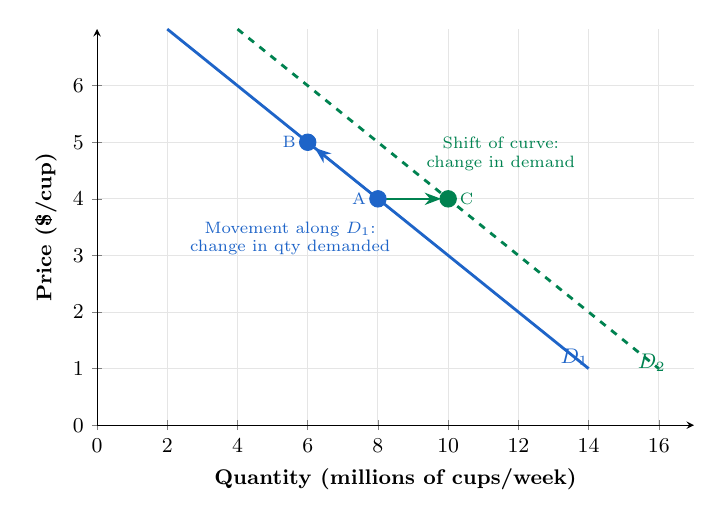
\begin{tikzpicture}[scale=0.85]
  \begin{axis}[
    width=10.5cm, height=7.5cm,
    xlabel={\textbf{Quantity} (millions of cups/week)},
    ylabel={\textbf{Price} (\$/cup)},
    xmin=0, xmax=17,
    ymin=0, ymax=7,
    xtick={0,2,4,6,8,10,12,14,16},
    ytick={0,1,2,3,4,5,6},
    tick label style={font=\small},
    label style={font=\small\bfseries},
    axis lines=left,
    grid=major, grid style={gray!20},
    clip=false,
  ]
  % D1 original
  \addplot[very thick, color=demandblue, domain=2:14, samples=2]
    {-0.5*x + 8};
  \node[font=\small\bfseries, color=demandblue] at (axis cs:13.6,1.2) {$D_1$};
  % D2 increase
  \addplot[very thick, color=leafgreen, domain=4:16, samples=2, dashed]
    {-0.5*x + 9};
  \node[font=\small\bfseries, color=leafgreen] at (axis cs:15.8,1.1) {$D_2$};
  % Movement along D1: points at P=4 and P=5
  \addplot[mark=*, mark size=3.5pt, color=demandblue] coordinates {(8,4)};
  \node[font=\scriptsize, color=demandblue, left] at (axis cs:7.9,4) {A};
  \addplot[mark=*, mark size=3.5pt, color=demandblue] coordinates {(6,5)};
  \node[font=\scriptsize, color=demandblue, left] at (axis cs:5.9,5) {B};
  % Arrow along D1
  \draw[-{Stealth[length=7pt]}, thick, color=demandblue]
    (axis cs:8,4) -- (axis cs:6.2,4.9);
  \node[font=\scriptsize, color=demandblue, align=center] at (axis cs:5.5,3.3)
    {Movement along $D_1$:\\change in qty demanded};
  % Shift arrow D1->D2
  \addplot[mark=*, mark size=3.5pt, color=leafgreen] coordinates {(10,4)};
  \node[font=\scriptsize, color=leafgreen, right] at (axis cs:10.1,4) {C};
  \draw[-{Stealth[length=7pt]}, thick, color=leafgreen]
    (axis cs:8,4) -- (axis cs:9.8,4);
  \node[font=\scriptsize, color=leafgreen, align=center] at (axis cs:11.5,4.8)
    {Shift of curve:\\change in demand};
  \end{axis}
\end{tikzpicture}
\end{center}
\end{frame}

\begin{frame}{Change in Demand vs.\ Change in Quantity Demanded}
\transfade
\begin{itemize}[<+->]
  \item A change in the \textbf{price of the product} causes a \textbf{movement along} the demand curve --- this is a \alert{change in quantity demanded}.
  \item Any other change affecting demand causes the \textbf{entire demand curve to shift} --- this is a \alert{change in demand}.
  \item \textbf{Common mistake:} saying ``the decrease in price causes demand to increase.'' The decrease in price causes a movement along the curve, not a shift.
\end{itemize}
\end{frame}

% ============================================================
\section{3.2 The Supply Side of the Market}
% ============================================================

\begin{frame}{3.2 Learning Objective}
\transfade
\begin{block}{Goal}
Discuss the variables that influence supply.
\end{block}
\begin{itemize}[<+->]
  \item Now we examine decisions of \textbf{firms}: how much of a product to provide at various prices.
  \item \textbf{Market supply:} the supply from all producers of a given good or service.
  \item We continue with the Tim Hortons medium coffee market.
\end{itemize}
\end{frame}

%--- FIG 3.4: Supply schedule + supply curve ---
\begin{frame}{Figure 3.4 -- Supply Schedule and Supply Curve}
\begin{columns}
\column{0.38\textwidth}
\centering
{\small\bfseries Tim Hortons Medium Coffee\\Supply Schedule}
\vspace{0.5em}

\renewcommand{\arraystretch}{1.4}
\begin{tabular}{cc}
\toprule
\textbf{\color{supplyred}Price} & \textbf{\color{supplyred}Qty Supplied}\\
(\$/cup) & (M cups/week)\\
\midrule
\$3.00 & 4 \\
\$3.50 & 6 \\
\$4.00 & 8 \\
\$4.50 & 10 \\
\$5.00 & 12 \\
\bottomrule
\end{tabular}
\vspace{0.5em}

{\scriptsize Source: Illustrative; based on\\Statistics Canada data}

\column{0.62\textwidth}
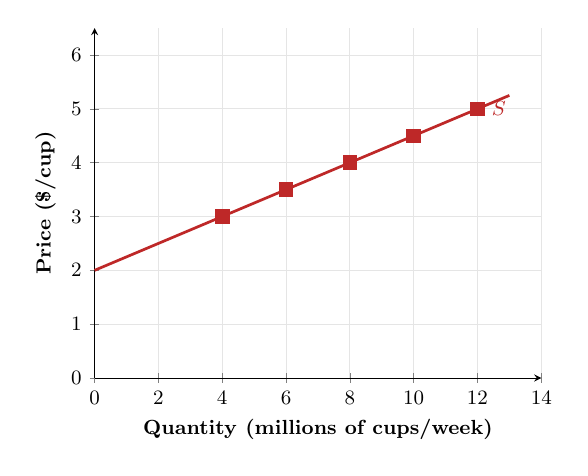
\begin{tikzpicture}[scale=0.82]
  \begin{axis}[
    width=8.5cm, height=7cm,
    xlabel={\textbf{Quantity} (millions of cups/week)},
    ylabel={\textbf{Price} (\$/cup)},
    xmin=0, xmax=14,
    ymin=0, ymax=6.5,
    xtick={0,2,4,6,8,10,12,14},
    ytick={0,1,2,3,4,5,6},
    tick label style={font=\small},
    label style={font=\small\bfseries},
    axis lines=left,
    grid=major, grid style={gray!20},
    clip=false,
  ]
  % Supply line: P = 0.25Q + 2
  \addplot[very thick, color=supplyred, domain=0:13, samples=2]
    {0.25*x + 2};
  \node[font=\small\bfseries, color=supplyred, right] at (axis cs:12.2,5) {$S$};
  % Data points
  \addplot[mark=square*, mark size=3pt, color=supplyred]
    coordinates {(4,3)(6,3.5)(8,4)(10,4.5)(12,5)};
  \end{axis}
\end{tikzpicture}
\end{columns}
\end{frame}

\begin{frame}{The Law of Supply}
\transfade
\begin{itemize}[<+->]
  \item \textbf{Quantity supplied:} the amount of a good a firm is willing and able to supply at a given price.
  \item \textbf{Law of supply:}
  \begin{itemize}[<+->]
    \item Holding everything else constant, increases in price cause \textbf{increases} in quantity supplied.
    \item Decreases in price cause \textbf{decreases} in quantity supplied.
  \end{itemize}
  \item \textbf{Why?} Higher prices make production more profitable, attracting more supply.
  \item \textbf{Canadian context:} When canola prices surged in 2021--2022, Prairie farmers allocated more acres to canola production (Statistics Canada, Field Crop Reporting Series).
\end{itemize}
\end{frame}

%--- FIG 3.5: Shifting the supply curve ---
\begin{frame}{Figure 3.5 -- Shifting the Supply Curve}
\begin{center}
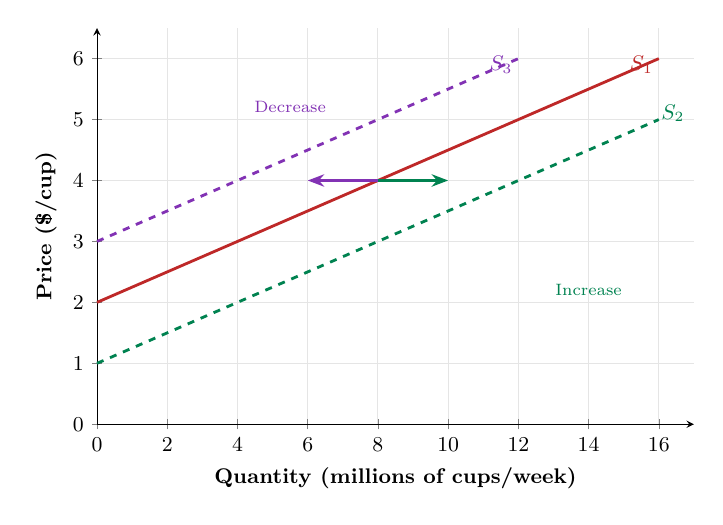
\begin{tikzpicture}[scale=0.85]
  \begin{axis}[
    width=10.5cm, height=7.5cm,
    xlabel={\textbf{Quantity} (millions of cups/week)},
    ylabel={\textbf{Price} (\$/cup)},
    xmin=0, xmax=17,
    ymin=0, ymax=6.5,
    xtick={0,2,4,6,8,10,12,14,16},
    ytick={0,1,2,3,4,5,6},
    tick label style={font=\small},
    label style={font=\small\bfseries},
    axis lines=left,
    grid=major, grid style={gray!20},
    clip=false,
  ]
  % S1 original: P = 0.25Q + 2
  \addplot[very thick, color=supplyred, domain=0:16, samples=2]
    {0.25*x + 2};
  \node[font=\small\bfseries, color=supplyred] at (axis cs:15.5,5.9) {$S_1$};
  % S2 increase (shift right): P = 0.25Q + 1
  \addplot[very thick, color=leafgreen, domain=0:16, samples=2, dashed]
    {0.25*x + 1};
  \node[font=\small\bfseries, color=leafgreen] at (axis cs:16.4,5.1) {$S_2$};
  \node[font=\scriptsize, color=leafgreen] at (axis cs:14,2.2) {Increase};
  % S3 decrease (shift left): P = 0.25Q + 3
  \addplot[very thick, color=shiftpurple, domain=0:12, samples=2, dashed]
    {0.25*x + 3};
  \node[font=\small\bfseries, color=shiftpurple] at (axis cs:11.5,5.9) {$S_3$};
  \node[font=\scriptsize, color=shiftpurple] at (axis cs:5.5,5.2) {Decrease};
  % Arrows
  \draw[-{Stealth[length=7pt]}, very thick, color=leafgreen]
    (axis cs:8,4) -- (axis cs:10,4);
  \draw[-{Stealth[length=7pt]}, very thick, color=shiftpurple]
    (axis cs:8,4) -- (axis cs:6,4);
  \end{axis}
\end{tikzpicture}
\end{center}
\end{frame}

\begin{frame}{Variables That Shift Market Supply}
\transfade
\begin{itemize}[<+->]
  \item \textbf{Prices of inputs} (labour, coffee beans, milk, paper cups)
  \item \textbf{Technological change} (brewing equipment efficiency)
  \item \textbf{Prices of substitutes in production}
  \item \textbf{Number of firms} in the market
  \item \textbf{Expected future prices}
\end{itemize}
\end{frame}

\begin{frame}{Changes in Prices of Inputs}
\transfade
\begin{itemize}[<+->]
  \item \textbf{Inputs:} anything used in production --- for coffee: arabica beans, milk, labour, paper cups, electricity.
  \item An \alert{increase} in input prices decreases profitability $\Rightarrow$ \textbf{decrease in supply} (curve shifts left).
  \item \textbf{Canadian example:} Global arabica coffee bean prices rose $\approx$70\% in 2024--2025 due to droughts in Brazil, raising costs for all Canadian coffee chains and reducing supply (ICO Coffee Report, 2025).
\end{itemize}
\end{frame}

\begin{frame}{Technological Change and Other Supply Shifters}
\transfade
\begin{itemize}[<+->]
  \item \textbf{Technological change:} new, more efficient brewing systems $\Rightarrow$ \textbf{increase in supply}.
  \item \textbf{Substitutes in production:} an Ontario farmer can plant corn or soybeans.
  \begin{itemize}[<+->]
    \item If soybean prices rise, farmers shift to soybeans $\Rightarrow$ \textbf{decrease in corn supply}.
  \end{itemize}
  \item \textbf{Complements in production:} beef and leather (more cattle farming raises supply of both).
  \item \textbf{Number of firms:} more coffee shops entering the market $\Rightarrow$ \textbf{increase in supply}.
  \item \textbf{Expected future prices:} if coffee prices expected to rise, firms may withhold supply now.
\end{itemize}
\end{frame}

%--- FIG 3.6: Change in supply vs. change in qty supplied ---
\begin{frame}{Figure 3.6 -- Change in Supply vs.\ Change in Quantity Supplied}
\begin{center}
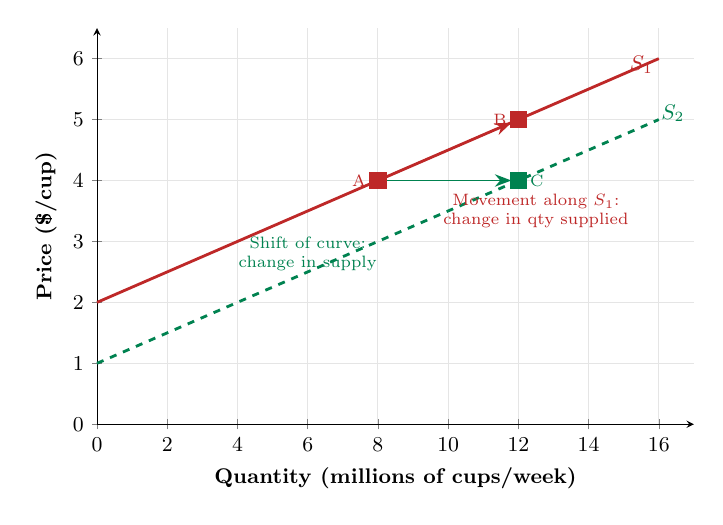
\begin{tikzpicture}[scale=0.85]
  \begin{axis}[
    width=10.5cm, height=7.5cm,
    xlabel={\textbf{Quantity} (millions of cups/week)},
    ylabel={\textbf{Price} (\$/cup)},
    xmin=0, xmax=17,
    ymin=0, ymax=6.5,
    xtick={0,2,4,6,8,10,12,14,16},
    ytick={0,1,2,3,4,5,6},
    tick label style={font=\small},
    label style={font=\small\bfseries},
    axis lines=left,
    grid=major, grid style={gray!20},
    clip=false,
  ]
  % S1
  \addplot[very thick, color=supplyred, domain=0:16, samples=2]
    {0.25*x + 2};
  \node[font=\small\bfseries, color=supplyred] at (axis cs:15.5,5.9) {$S_1$};
  % S2 increase
  \addplot[very thick, color=leafgreen, domain=0:16, samples=2, dashed]
    {0.25*x + 1};
  \node[font=\small\bfseries, color=leafgreen] at (axis cs:16.4,5.1) {$S_2$};
  % Points for movement along S1: A at (8,4), B at (12,5)
  \addplot[mark=square*, mark size=3.5pt, color=supplyred] coordinates {(8,4)};
  \node[font=\scriptsize, color=supplyred, left] at (axis cs:7.9,4) {A};
  \addplot[mark=square*, mark size=3.5pt, color=supplyred] coordinates {(12,5)};
  \node[font=\scriptsize, color=supplyred, left] at (axis cs:11.9,5) {B};
  \draw[-{Stealth[length=7pt]}, thick, color=supplyred]
    (axis cs:8,4) -- (axis cs:11.8,4.95);
  \node[font=\scriptsize, color=supplyred, align=center] at (axis cs:12.5,3.5)
    {Movement along $S_1$:\\change in qty supplied};
  % Point on S2 for shift
  \addplot[mark=square*, mark size=3.5pt, color=leafgreen] coordinates {(12,4)};
  \node[font=\scriptsize, color=leafgreen, right] at (axis cs:12.1,4) {C};
  \draw[-{Stealth[length=7pt]}, thick, color=leafgreen]
    (axis cs:8,4) -- (axis cs:11.8,4);
  \node[font=\scriptsize, color=leafgreen, align=center] at (axis cs:6,2.8)
    {Shift of curve:\\change in supply};
  \end{axis}
\end{tikzpicture}
\end{center}
\end{frame}

% ============================================================
\section{3.3 Market Equilibrium}
% ============================================================

\begin{frame}{3.3 Learning Objective}
\transfade
\begin{block}{Goal}
Use a graph to illustrate market equilibrium.
\end{block}
\begin{itemize}[<+->]
  \item \textbf{Market equilibrium:} quantity demanded equals quantity supplied.
  \item In perfectly competitive markets, this is called a \textbf{competitive market equilibrium}.
  \item The equilibrium price is the price that \emph{clears} the market.
\end{itemize}
\end{frame}

%--- FIG 3.7: Market equilibrium ---
\begin{frame}{Figure 3.7 -- Market Equilibrium: Tim Hortons Coffee}
\begin{center}
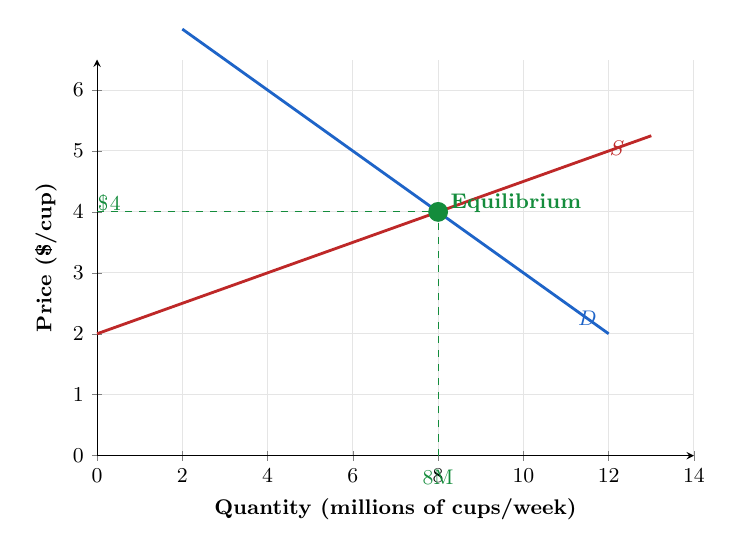
\begin{tikzpicture}[scale=0.85]
  \begin{axis}[
    width=10.5cm, height=7.5cm,
    xlabel={\textbf{Quantity} (millions of cups/week)},
    ylabel={\textbf{Price} (\$/cup)},
    xmin=0, xmax=14,
    ymin=0, ymax=6.5,
    xtick={0,2,4,6,8,10,12,14},
    ytick={0,1,2,3,4,5,6},
    tick label style={font=\small},
    label style={font=\small\bfseries},
    axis lines=left,
    grid=major, grid style={gray!20},
    clip=false,
  ]
  % Demand: P = -0.5Q + 8
  \addplot[very thick, color=demandblue, domain=2:12, samples=2]
    {-0.5*x + 8};
  \node[font=\small\bfseries, color=demandblue] at (axis cs:11.5,2.25) {$D$};
  % Supply: P = 0.25Q + 2
  \addplot[very thick, color=supplyred, domain=0:13, samples=2]
    {0.25*x + 2};
  \node[font=\small\bfseries, color=supplyred] at (axis cs:12.2,5.05) {$S$};
  % Equilibrium point
  \addplot[mark=*, mark size=4pt, color=eqgreen] coordinates {(8,4)};
  \node[font=\small\bfseries, color=eqgreen, right] at (axis cs:8.1,4.15)
    {Equilibrium};
  % Dashed lines to axes
  \addplot[dashed, color=eqgreen, domain=0:8, samples=2] {4};
  \draw[dashed, color=eqgreen] (axis cs:8,0) -- (axis cs:8,4);
  \node[font=\small, color=eqgreen] at (axis cs:0.3,4.15) {\$4};
  \node[font=\small, color=eqgreen] at (axis cs:8,-0.35) {8M};
  \end{axis}
\end{tikzpicture}
\end{center}
\end{frame}

\begin{frame}{Reading the Equilibrium}
\transfade
\begin{itemize}[<+->]
  \item At a price of \textbf{\$4.00/cup}:
  \begin{itemize}[<+->]
    \item Consumers want to buy \textbf{8 million} cups/week.
    \item Producers want to sell \textbf{8 million} cups/week.
  \end{itemize}
  \item The \textbf{equilibrium price} is \$4.00/cup; the \textbf{equilibrium quantity} is 8 million cups/week.
  \item At any other price, the market is out of balance --- either a surplus or a shortage exists.
\end{itemize}
\end{frame}

%--- FIG 3.8: Surplus and shortage ---
\begin{frame}{Figure 3.8 -- Surplus and Shortage}
\begin{center}
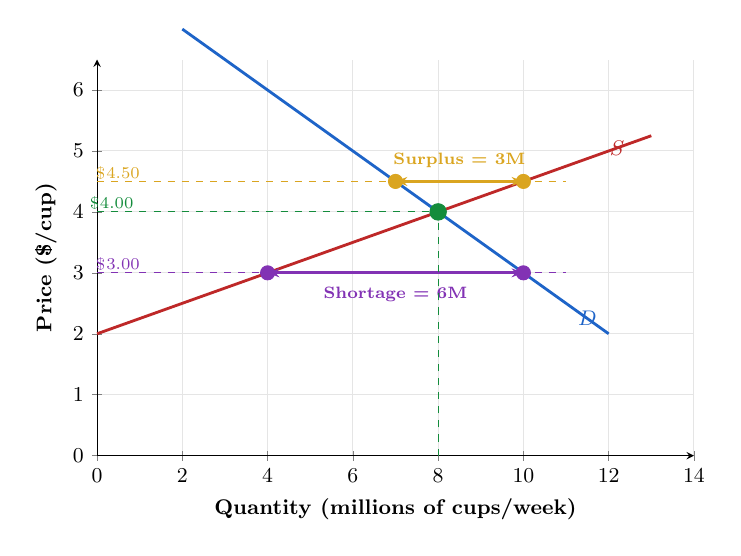
\begin{tikzpicture}[scale=0.85]
  \begin{axis}[
    width=10.5cm, height=7.5cm,
    xlabel={\textbf{Quantity} (millions of cups/week)},
    ylabel={\textbf{Price} (\$/cup)},
    xmin=0, xmax=14,
    ymin=0, ymax=6.5,
    xtick={0,2,4,6,8,10,12,14},
    ytick={0,1,2,3,4,5,6},
    tick label style={font=\small},
    label style={font=\small\bfseries},
    axis lines=left,
    grid=major, grid style={gray!20},
    clip=false,
  ]
  % D and S
  \addplot[very thick, color=demandblue, domain=2:12, samples=2] {-0.5*x + 8};
  \node[font=\small\bfseries, color=demandblue] at (axis cs:11.5,2.25) {$D$};
  \addplot[very thick, color=supplyred, domain=0:13, samples=2] {0.25*x + 2};
  \node[font=\small\bfseries, color=supplyred] at (axis cs:12.2,5.05) {$S$};
  % Equilibrium
  \addplot[mark=*, mark size=3.5pt, color=eqgreen] coordinates {(8,4)};
  % Surplus at P=4.50: Qd=7, Qs=10
  \draw[dashed, color=goldenrod] (axis cs:0,4.5) -- (axis cs:11,4.5);
  \addplot[mark=*, mark size=3pt, color=goldenrod] coordinates {(7,4.5)(10,4.5)};
  \draw[{Stealth[length=5pt]}-{Stealth[length=5pt]}, very thick, color=goldenrod]
    (axis cs:7,4.5) -- (axis cs:10,4.5);
  \node[font=\scriptsize\bfseries, color=goldenrod] at (axis cs:8.5,4.85)
    {Surplus = 3M};
  \node[font=\scriptsize, color=goldenrod] at (axis cs:0.5,4.65) {\$4.50};
  % Shortage at P=3.00: Qd=10, Qs=4
  \draw[dashed, color=shiftpurple] (axis cs:0,3) -- (axis cs:11,3);
  \addplot[mark=*, mark size=3pt, color=shiftpurple] coordinates {(4,3)(10,3)};
  \draw[{Stealth[length=5pt]}-{Stealth[length=5pt]}, very thick, color=shiftpurple]
    (axis cs:4,3) -- (axis cs:10,3);
  \node[font=\scriptsize\bfseries, color=shiftpurple] at (axis cs:7,2.65)
    {Shortage = 6M};
  \node[font=\scriptsize, color=shiftpurple] at (axis cs:0.5,3.15) {\$3.00};
  % Eq dashes
  \draw[dashed, color=eqgreen] (axis cs:0,4) -- (axis cs:8,4);
  \draw[dashed, color=eqgreen] (axis cs:8,0) -- (axis cs:8,4);
  \node[font=\scriptsize, color=eqgreen] at (axis cs:0.35,4.15) {\$4.00};
  \end{axis}
\end{tikzpicture}
\end{center}
\end{frame}

\begin{frame}{Surplus and Shortage}
\transfade
\begin{itemize}[<+->]
  \item \textbf{Surplus} (P = \$4.50): $Q_s = 10\text{M} > Q_d = 7\text{M}$ --- surplus of 3M cups/week.
  \begin{itemize}[<+->]
    \item Sellers compete among themselves $\Rightarrow$ price is bid \textbf{down} toward \$4.00.
  \end{itemize}
  \item \textbf{Shortage} (P = \$3.00): $Q_d = 10\text{M} > Q_s = 4\text{M}$ --- shortage of 6M cups/week.
  \begin{itemize}[<+->]
    \item Buyers compete among themselves $\Rightarrow$ price is bid \textbf{up} toward \$4.00.
  \end{itemize}
  \item Price is determined by the \textbf{interaction} of buyers and sellers --- neither group alone controls it.
\end{itemize}
\end{frame}

% ============================================================
\section{3.4 Shifts in Demand and Supply}
% ============================================================

\begin{frame}{3.4 Learning Objective}
\transfade
\begin{block}{Goal}
Use demand and supply graphs to predict changes in prices and quantities.
\end{block}
\begin{itemize}[<+->]
  \item We typically observe the current price and quantity, but do \emph{not} observe the whole curves.
  \item The model predicts \textbf{directional} changes in price and quantity when curves shift.
\end{itemize}
\end{frame}

%--- FIG 3.9: Supply increases ---
\begin{frame}{Figure 3.9 -- Effect of an Increase in Supply}
\begin{center}
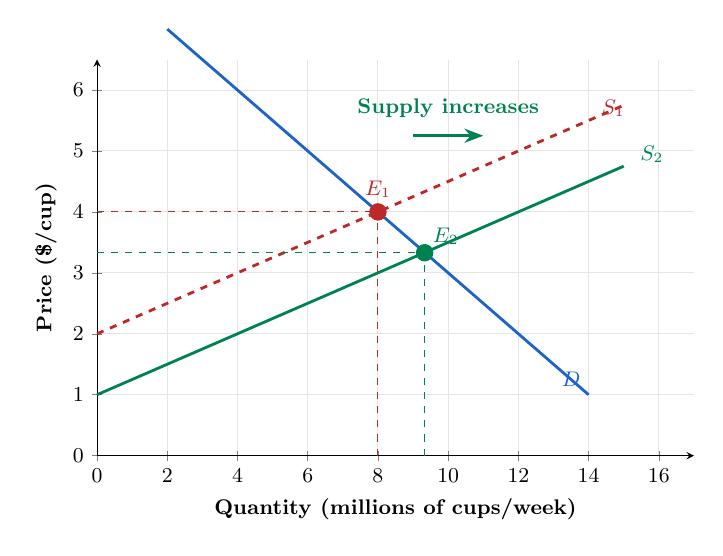
\begin{tikzpicture}[scale=0.85]
  \begin{axis}[
    width=10.5cm, height=7.5cm,
    xlabel={\textbf{Quantity} (millions of cups/week)},
    ylabel={\textbf{Price} (\$/cup)},
    xmin=0, xmax=17,
    ymin=0, ymax=6.5,
    xtick={0,2,4,6,8,10,12,14,16},
    ytick={0,1,2,3,4,5,6},
    tick label style={font=\small},
    label style={font=\small\bfseries},
    axis lines=left,
    grid=major, grid style={gray!20},
    clip=false,
  ]
  % D unchanged
  \addplot[very thick, color=demandblue, domain=2:14, samples=2] {-0.5*x + 8};
  \node[font=\small\bfseries, color=demandblue] at (axis cs:13.5,1.25) {$D$};
  % S1 original
  \addplot[very thick, color=supplyred, domain=0:15, samples=2, dashed] {0.25*x + 2};
  \node[font=\small\bfseries, color=supplyred] at (axis cs:14.7,5.7) {$S_1$};
  % S2 increase (shift right: P = 0.25Q + 1)
  \addplot[very thick, color=leafgreen, domain=0:15, samples=2] {0.25*x + 1};
  \node[font=\small\bfseries, color=leafgreen] at (axis cs:15.8,4.95) {$S_2$};
  % Eq1: S1 and D: -0.5Q+8=0.25Q+2 -> 6=0.75Q -> Q=8, P=4
  \addplot[mark=*, mark size=3.5pt, color=supplyred] coordinates {(8,4)};
  \node[font=\small\bfseries, color=supplyred, above] at (axis cs:8,4.1) {$E_1$};
  % Eq2: S2 and D: -0.5Q+8=0.25Q+1 -> 7=0.75Q -> Q=9.33, P=3.33
  \addplot[mark=*, mark size=3.5pt, color=leafgreen] coordinates {(9.33,3.33)};
  \node[font=\small\bfseries, color=leafgreen, above right] at (axis cs:9.33,3.33) {$E_2$};
  % Dashes
  \draw[dashed, color=supplyred] (axis cs:0,4) -- (axis cs:8,4);
  \draw[dashed, color=supplyred] (axis cs:8,0) -- (axis cs:8,4);
  \draw[dashed, color=leafgreen] (axis cs:0,3.33) -- (axis cs:9.33,3.33);
  \draw[dashed, color=leafgreen] (axis cs:9.33,0) -- (axis cs:9.33,3.33);
  % Arrow
  \draw[-{Stealth[length=8pt]}, very thick, color=leafgreen]
    (axis cs:9,5.25) -- (axis cs:11,5.25);
  \node[font=\small\bfseries, color=leafgreen] at (axis cs:10,5.7) {Supply increases};
  \end{axis}
\end{tikzpicture}
\end{center}
\end{frame}

\begin{frame}{Effect of an Increase in Supply}
\transfade
\begin{itemize}[<+->]
  \item New coffee chains enter the Canadian market (e.g., Dutch Bros. expanding into Canada).
  \item Supply shifts \textbf{right} from $S_1$ to $S_2$.
  \item \textbf{Result:}
  \begin{itemize}[<+->]
    \item Equilibrium price \textbf{falls} (\$4.00 $\to$ \$3.33).
    \item Equilibrium quantity \textbf{rises} (8M $\to$ 9.3M cups/week).
  \end{itemize}
  \item We only predict \emph{directions} --- the exact magnitude requires knowing the full curves.
\end{itemize}
\end{frame}

%--- FIG 3.10: Demand increases ---
\begin{frame}{Figure 3.10 -- Effect of an Increase in Demand}
\begin{center}
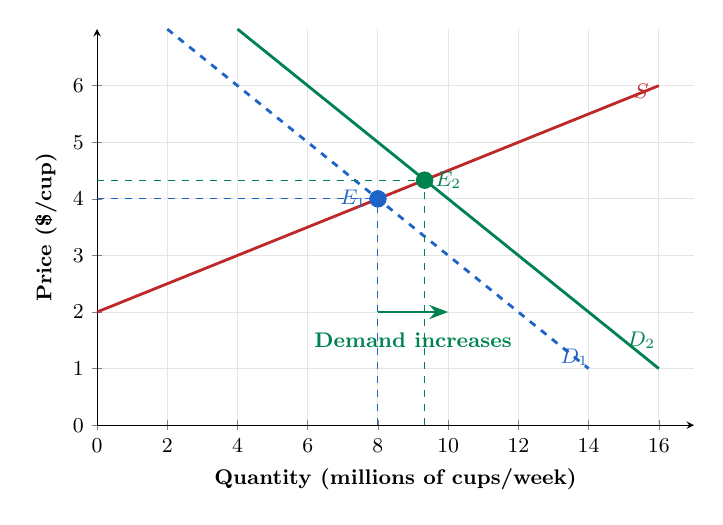
\begin{tikzpicture}[scale=0.85]
  \begin{axis}[
    width=10.5cm, height=7.5cm,
    xlabel={\textbf{Quantity} (millions of cups/week)},
    ylabel={\textbf{Price} (\$/cup)},
    xmin=0, xmax=17,
    ymin=0, ymax=7,
    xtick={0,2,4,6,8,10,12,14,16},
    ytick={0,1,2,3,4,5,6},
    tick label style={font=\small},
    label style={font=\small\bfseries},
    axis lines=left,
    grid=major, grid style={gray!20},
    clip=false,
  ]
  % S unchanged
  \addplot[very thick, color=supplyred, domain=0:16, samples=2] {0.25*x + 2};
  \node[font=\small\bfseries, color=supplyred] at (axis cs:15.5,5.9) {$S$};
  % D1 original
  \addplot[very thick, color=demandblue, domain=2:14, samples=2, dashed] {-0.5*x + 8};
  \node[font=\small\bfseries, color=demandblue] at (axis cs:13.6,1.2) {$D_1$};
  % D2 increase: P = -0.5Q + 9
  \addplot[very thick, color=leafgreen, domain=4:16, samples=2] {-0.5*x + 9};
  \node[font=\small\bfseries, color=leafgreen] at (axis cs:15.5,1.5) {$D_2$};
  % Eq1: Q=8, P=4
  \addplot[mark=*, mark size=3.5pt, color=demandblue] coordinates {(8,4)};
  \node[font=\small\bfseries, color=demandblue, left] at (axis cs:7.9,4) {$E_1$};
  % Eq2: -0.5Q+9=0.25Q+2 -> 7=0.75Q -> Q=9.33, P=4.33
  \addplot[mark=*, mark size=3.5pt, color=leafgreen] coordinates {(9.33,4.33)};
  \node[font=\small\bfseries, color=leafgreen, right] at (axis cs:9.4,4.33) {$E_2$};
  % Dashes
  \draw[dashed, color=demandblue] (axis cs:0,4) -- (axis cs:8,4);
  \draw[dashed, color=demandblue] (axis cs:8,0) -- (axis cs:8,4);
  \draw[dashed, color=leafgreen] (axis cs:0,4.33) -- (axis cs:9.33,4.33);
  \draw[dashed, color=leafgreen] (axis cs:9.33,0) -- (axis cs:9.33,4.33);
  % Arrow
  \draw[-{Stealth[length=8pt]}, very thick, color=leafgreen]
    (axis cs:8,2) -- (axis cs:10,2);
  \node[font=\small\bfseries, color=leafgreen] at (axis cs:9,1.5) {Demand increases};
  \end{axis}
\end{tikzpicture}
\end{center}
\end{frame}

\begin{frame}{Effect of an Increase in Demand}
\transfade
\begin{itemize}[<+->]
  \item Canada's population grew by $\approx$3 million in 2022--2024 (Statistics Canada) --- more coffee drinkers.
  \item Demand shifts \textbf{right} from $D_1$ to $D_2$.
  \item \textbf{Result:}
  \begin{itemize}[<+->]
    \item Equilibrium price \textbf{rises} (\$4.00 $\to$ \$4.33).
    \item Equilibrium quantity \textbf{rises} (8M $\to$ 9.3M cups/week).
  \end{itemize}
  \item Both price and quantity increase when demand increases and supply is unchanged.
\end{itemize}
\end{frame}

%--- TABLE 3.3: Summary of shifts ---
\begin{frame}{Table 3.3 -- How Shifts Affect Equilibrium $P$ and $Q$}
\begin{center}
\renewcommand{\arraystretch}{1.5}
\begin{tabular}{lcc}
\toprule
\textbf{Change} & \textbf{Eq.\ Price $P$} & \textbf{Eq.\ Quantity $Q$} \\
\midrule
Demand $\uparrow$, supply unchanged & \textcolor{leafgreen}{Rises} & \textcolor{leafgreen}{Rises} \\
Demand $\downarrow$, supply unchanged & \textcolor{canadared}{Falls} & \textcolor{canadared}{Falls} \\
Supply $\uparrow$, demand unchanged & \textcolor{canadared}{Falls} & \textcolor{leafgreen}{Rises} \\
Supply $\downarrow$, demand unchanged & \textcolor{leafgreen}{Rises} & \textcolor{canadared}{Falls} \\
\midrule
Demand $\uparrow$ and supply $\downarrow$ & \textcolor{leafgreen}{Rises} & \textbf{?} \\
Demand $\downarrow$ and supply $\uparrow$ & \textcolor{canadared}{Falls} & \textbf{?} \\
Demand $\uparrow$ and supply $\uparrow$ & \textbf{?} & \textcolor{leafgreen}{Rises} \\
Demand $\downarrow$ and supply $\downarrow$ & \textbf{?} & \textcolor{canadared}{Falls} \\
\bottomrule
\end{tabular}
\end{center}
\vspace{0.3em}
{\small \textbf{?} = ambiguous: the direction depends on the \emph{relative} size of the shifts.}
\end{frame}

%--- FIG 3.11: Both curves shift ---
\begin{frame}{Figure 3.11 -- Both Demand and Supply Shift}
\begin{columns}
\column{0.5\textwidth}
\centering
{\small\bfseries\color{accent} Case 1: Demand shifts more}
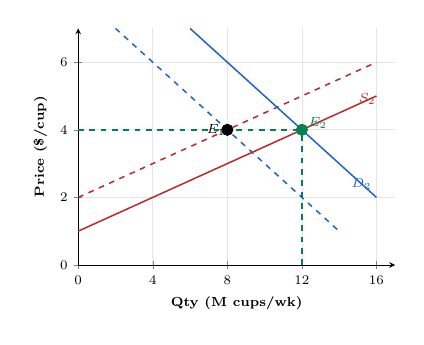
\begin{tikzpicture}[scale=0.68]
  \begin{axis}[
    width=7.5cm, height=6cm,
    xlabel={Qty (M cups/wk)},
    ylabel={Price (\$/cup)},
    xmin=0, xmax=17,
    ymin=0, ymax=7,
    xtick={0,4,8,12,16},
    ytick={0,2,4,6},
    tick label style={font=\scriptsize},
    label style={font=\scriptsize\bfseries},
    axis lines=left,
    grid=major, grid style={gray!20},
    clip=false,
  ]
  % D1, S1
  \addplot[thick, color=demandblue, dashed, domain=2:14, samples=2] {-0.5*x+8};
  \addplot[thick, color=supplyred, dashed, domain=0:16, samples=2] {0.25*x+2};
  % D2 big shift: P=-0.5Q+10
  \addplot[thick, color=demandblue, domain=6:16, samples=2] {-0.5*x+10};
  \node[font=\scriptsize\bfseries, color=demandblue] at (axis cs:15.2,2.4) {$D_2$};
  % S2 small shift: P=0.25Q+1
  \addplot[thick, color=supplyred, domain=0:16, samples=2] {0.25*x+1};
  \node[font=\scriptsize\bfseries, color=supplyred] at (axis cs:15.5,4.9) {$S_2$};
  % Eq1: Q=8, P=4
  \addplot[mark=*, mark size=3pt, color=black] coordinates {(8,4)};
  \node[font=\scriptsize\bfseries] at (axis cs:7.4,4) {$E_1$};
  % Eq2: -0.5Q+10=0.25Q+1 -> 9=0.75Q -> Q=12, P=4
  \addplot[mark=*, mark size=3pt, color=leafgreen] coordinates {(12,4)};
  \node[font=\scriptsize\bfseries, color=leafgreen, right] at (axis cs:12,4.2) {$E_2$};
  \draw[dashed, thick, color=leafgreen] (axis cs:0,4) -- (axis cs:12,4);
  \draw[dashed, thick, color=leafgreen] (axis cs:12,0) -- (axis cs:12,4);
  \end{axis}
\end{tikzpicture}

\column{0.5\textwidth}
\centering
{\small\bfseries\color{canadared} Case 2: Supply shifts more}
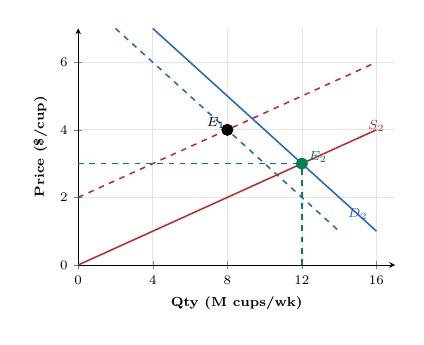
\begin{tikzpicture}[scale=0.68]
  \begin{axis}[
    width=7.5cm, height=6cm,
    xlabel={Qty (M cups/wk)},
    ylabel={Price (\$/cup)},
    xmin=0, xmax=17,
    ymin=0, ymax=7,
    xtick={0,4,8,12,16},
    ytick={0,2,4,6},
    tick label style={font=\scriptsize},
    label style={font=\scriptsize\bfseries},
    axis lines=left,
    grid=major, grid style={gray!20},
    clip=false,
  ]
  % D1, S1
  \addplot[thick, color=demandblue, dashed, domain=2:14, samples=2] {-0.5*x+8};
  \addplot[thick, color=supplyred, dashed, domain=0:16, samples=2] {0.25*x+2};
  % D2 small shift: P=-0.5Q+9
  \addplot[thick, color=demandblue, domain=4:16, samples=2] {-0.5*x+9};
  \node[font=\scriptsize\bfseries, color=demandblue] at (axis cs:15,1.5) {$D_2$};
  % S2 big shift: P=0.25Q+0
  \addplot[thick, color=supplyred, domain=0:16, samples=2] {0.25*x};
  \node[font=\scriptsize\bfseries, color=supplyred] at (axis cs:16,4.1) {$S_2$};
  % Eq1: Q=8, P=4
  \addplot[mark=*, mark size=3pt, color=black] coordinates {(8,4)};
  \node[font=\scriptsize\bfseries] at (axis cs:7.4,4.2) {$E_1$};
  % Eq2: -0.5Q+9=0.25Q -> 9=0.75Q -> Q=12, P=3
  \addplot[mark=*, mark size=3pt, color=leafgreen] coordinates {(12,3)};
  \node[font=\scriptsize\bfseries, color=leafgreen, right] at (axis cs:12,3.2) {$E_2$};
  \draw[dashed, thick, color=leafgreen] (axis cs:0,3) -- (axis cs:12,3);
  \draw[dashed, thick, color=leafgreen] (axis cs:12,0) -- (axis cs:12,3);
  \end{axis}
\end{tikzpicture}
\end{columns}
\vspace{0.3em}
\centering\small Both cases: quantity \textbf{rises}. Price: \textbf{ambiguous} --- depends on which shift is larger.
\end{frame}

\begin{frame}{Shifts of Curves vs.\ Movements Along Curves}
\transfade
\begin{itemize}[<+->]
  \item Suppose an \textbf{increase in supply} occurs.
  \begin{itemize}[<+->]
    \item Equilibrium quantity increases; equilibrium price decreases.
  \end{itemize}
  \item It is tempting to say ``the decrease in price causes an increase in demand'' --- \textbf{incorrect}.
  \item The decrease in price causes a \textbf{movement along the demand curve}, not a shift.
  \item The demand curve already describes how much consumers want to buy at \textbf{any given price}.
  \item \textbf{Canadian example:} When new discount airlines entered the YVR--YYZ route, fares fell and more passengers flew --- that is a movement along demand, not a demand shift.
\end{itemize}
\end{frame}

% ============================================================
\section{Chapter Summary}
% ============================================================

\begin{frame}{Things to Remember}
\transfade
\begin{itemize}[<+->]
  \item A \textbf{change in price} causes a movement \textbf{along} the demand or supply curve.
  \item Any \textbf{other change} shifts the entire curve.
  \item In equilibrium, $Q_d = Q_s$; surpluses push price \textbf{down}; shortages push price \textbf{up}.
  \item When both curves shift, one effect is \textbf{ambiguous} --- need to know relative magnitudes.
  \item Markets coordinate millions of buyers and sellers through prices --- no central planner required.
\end{itemize}
\end{frame}

\begin{frame}{Chapter Summary}
\transfade
\begin{itemize}[<+->]
  \item \textbf{Demand} follows the law of demand; explained by substitution and income effects. Shifts when income, prices of related goods, tastes, population, or expectations change.
  \item \textbf{Supply} follows the law of supply. Shifts when input prices, technology, production substitutes/complements, number of firms, or expected future prices change.
  \item \textbf{Market equilibrium} occurs where $Q_d = Q_s$. Surpluses drive price down; shortages drive it up.
  \item The demand and supply model predicts \textbf{directional} changes in equilibrium $P$ and $Q$ when curves shift.
  \item \textbf{Data:} Statistics Canada CPI, Bank of Canada, Restaurant Brands International earnings.
\end{itemize}
\end{frame}

\begin{frame}
\centering
\Huge \textbf{Thank you!}\\[1em]
\normalsize Questions?\\[0.5em]
\small \textit{Data sources: Statistics Canada, Bank of Canada, NRCan, Restaurant Brands International}
\end{frame}

\end{document}
